% !TEX root = ../tjumain.tex

\chapter{总体设计}

根据TCP协议具有的功能和实践内容结合,本次实验的协议设计分为以下三个部分,分别是连接管理和流量控制、可靠数据传输和拥塞控制。

\section{可靠数据传输相关设计}

为了向应用层提供可靠的端到端数据传输服务。我们需要有 连接建立、数据传输、连接关闭 三个方面的功能。在本次实验中,我们首先在第一周完成了连接建立的过程,即通过三次握手完成 TCP 连接的建立。本周,我们将重点完成第二个功能,即可靠的数据传输服务。

相关的API如下:
\begin{enumerate}
  \item Client \begin{enumerate}
    \item int tju\_send(...): 将应用层的信息放入发送缓冲区,并进行发送。
  \end{enumerate}
  \item Server \begin{enumerate}
    \item int tju\_recv(...): 接收由 handle\_packet 等函数放入接收缓冲区的信息
  \end{enumerate}
  \item 通用 \begin{enumerate}
      \item tju\_tcp\_t * tju\_socket(): 创建 socket 并初始化数据结构(包括发送、接收缓冲区等),根据本周的要求,还增加了关于时钟初始化、trace 文件初始化等操作,最终返回 socket 的指针
      \item tju\_handle\_packet(): 处理接收到的包裹。在 Established 状态下,根据接收缓冲区的大小,选择性的将不按顺序到来的包裹放入接收树(自定义数据结构)或者丢弃。并在接收到正确包裹时,将树中正确的包裹按顺序放入缓冲区中等待应用层获取。
  \end{enumerate}
\end{enumerate}

\section{模块功能设计}

\begin{figure}[!htbp]
  \centering
  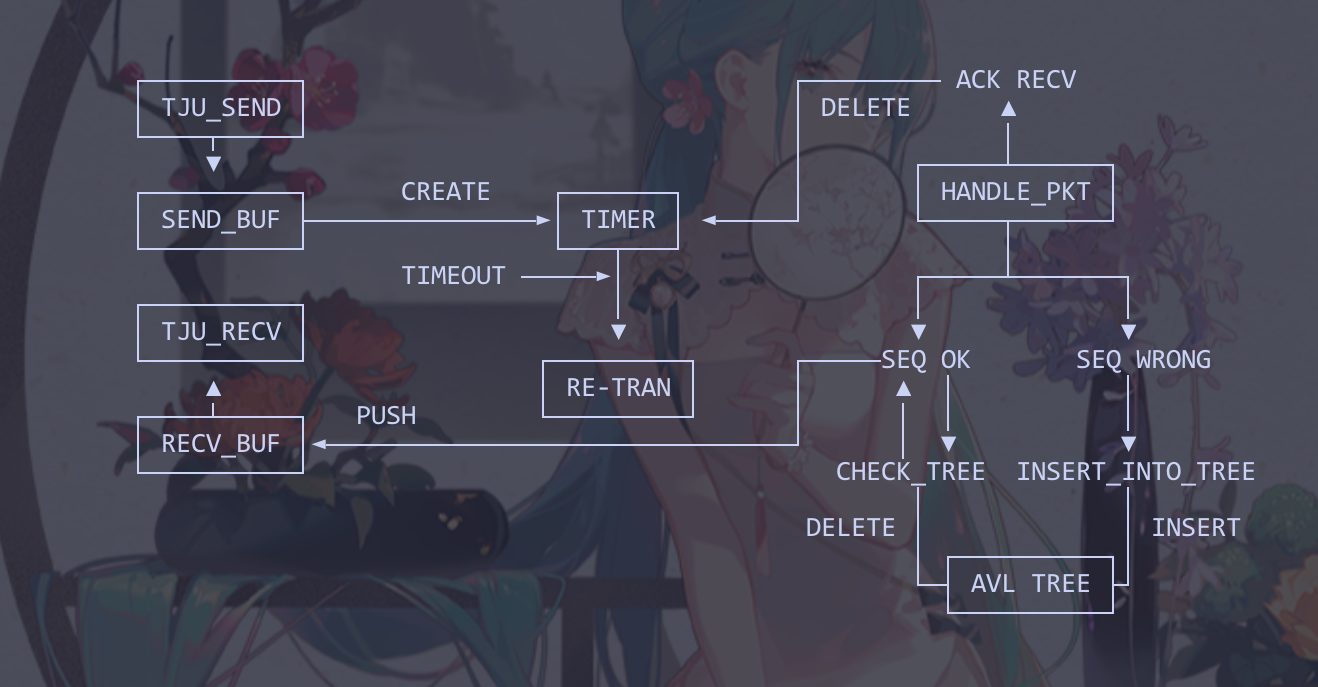
\includegraphics[width=.8\textwidth]{figures/Flow_10_4.png}
  \label{fig:flow}\caption{可靠数据传输相关功能设计总览}
\end{figure}

从图中可以看到,我们通过一个 TIMER 线程专门检查所有 registered TIMER 并在其 TIMEOUT 时执行 RE-TRAN,即重传。同时,我们在 HANDLE\_PACKET 函数,在收到 ACK 时,关闭响应的 TIMER(TIMER的实现采用 queue 的数据结构,确保快速增删)。

对于 Server 端,我们在 HANDLE\_PACKET 中设计了根据 SEQ number 的检验功能,当 SEQ number 正确时,我们直接将内容放入缓冲区,否则将其放入一颗 AVL 树中等待正确 SEQ 达到后,再进行查找并放入缓冲区,确保缓冲区中的内容都是连贯一致的。


